

\begin{frame}
    \frametitle{Exercise 3.4 - 15}
    \textit{Problem Statement}\\
    Let \(\topx\) be a \emph{finite} topological space. Show that the following are
    equivalent:
    \begin{enumerate}
        \item \(\topx\) has the discrete topology.
        \item \(\topx\) is metrizable.
        \item \(\topx\) is Hausdorff.
    \end{enumerate}
\end{frame}

\begin{frame}
    \frametitle{Establishing Relationships}
    \centering
    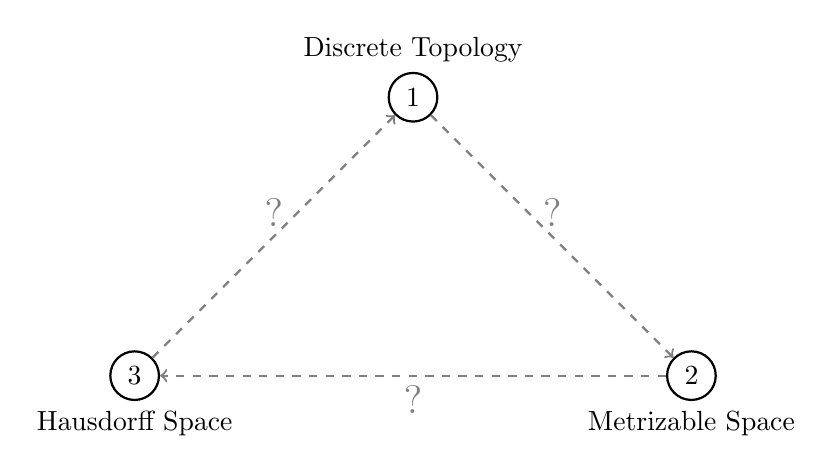
\begin{tikzpicture}[node distance={5cm}, thick, main/.style = {draw, circle}]
        \node[main, label=above:Discrete Topology] (1)                      {\(1\)};
        \node[main, label=below:Metrizable Space] (2) [below right of=1]    {\(2\)};
        \node[main, label=below:Hausdorff Space] (3) [below left of=1]      {\(3\)};

        % \pause

        \draw[->, color=gray] (1) -- node[midway, above] {\Large ?} (2) [dashed];
        \draw[->, color=gray] (2) -- node[midway, below] {\Large ?} (3) [dashed];
        \draw[->, color=gray] (3) -- node[midway, above] {\Large ?} (1) [dashed];

    \end{tikzpicture}

\end{frame}

\begin{frame}
    \frametitle{\(1 \rightarrow 2\) --- Discrete \(\rightarrow\) Metrizable}

    % discrete space
    % \begin{figure}
    %     \scalebox{1.4}{\input{fig/sankalp/metrizable.pdf_tex}}
    % \end{figure}

    We've already seen this done by Parth. We choose the discrete metric 

    \begin{columns}
        \begin{column}{0.5\textwidth}
            \begin{gather*}
                \topx \in \textsf{Metric}\\
                d : \topx \times \topx \to \reals 
            \end{gather*}
        \end{column}
        \begin{column}{0.5\textwidth}
            \begin{gather*}
                d(x, y) = \begin{cases}
                    1 \text{ if } x \not = y,\\
                    0 \text{ otherwise.}
                \end{cases}
            \end{gather*}
        \end{column}
    \end{columns}

    \pause

    \begin{figure}
        \scalebox{1}{\input{fig/sankalp/discrete.pdf_tex}}
    \end{figure}

\end{frame}

\begin{frame}
    \frametitle{\(2 \rightarrow 3\) --- Metrizable \(\rightarrow\) Hausdorff}

    % metrizable, existence of metric
    Given that the space, say \((\topx, \tau)\), is metrizable, there exists a
    metric \(d: \topx \times \topx \to \reals\) which induces the topology given
    by \(\tau\). \pause
    %
    % construct ball and shrink
    Use this metric to define open balls \(B_i, B_j\) for any pair of points in
    \(\topx, x_i, x_j\). \pause By shrinking these open balls, we can create
    non-intersecting open sets as required.
    %
    \pause
    %
    \begin{figure}
        \scalebox{1}{\input{fig/sankalp/separable.pdf_tex}}
    \end{figure}

\end{frame}

\begin{frame}
    \frametitle{\(3 \rightarrow 1\) --- Hausdorff \(\rightarrow\) Discrete}

    % construct Hausdorff sets
    We know by the Hausdorff property that any two points are separable by
    neighbourhoods.

    \pause

    % show point exclusion

    \begin{columns}
        \begin{column}{0.5\textwidth}
            \begin{figure}
                \scalebox{1}{%LaTeX with PSTricks extensions
%%Creator: Inkscape 1.1 (c4e8f9ed74, 2021-05-24)
%%Please note this file requires PSTricks extensions
\psset{xunit=.5pt,yunit=.5pt,runit=.5pt}
\begin{pspicture}(261.52766671,199.02523491)
{
\newrgbcolor{curcolor}{1 0.90196079 0.83529413}
\pscustom[linestyle=none,fillstyle=solid,fillcolor=curcolor]
{
\newpath
\moveto(250.93652409,86.60347491)
\curveto(211.63763528,112.81625602)(37.86237732,40.83746672)(142.27548472,3.98562546)
\curveto(190.07341228,-12.8842958)(293.64317102,34.46429507)(250.93652409,86.60347491)
\closepath
}
}
{
\newrgbcolor{curcolor}{1 0.40000001 0}
\pscustom[linewidth=0.99999871,linecolor=curcolor]
{
\newpath
\moveto(250.93652409,86.60347491)
\curveto(211.63763528,112.81625602)(37.86237732,40.83746672)(142.27548472,3.98562546)
\curveto(190.07341228,-12.8842958)(293.64317102,34.46429507)(250.93652409,86.60347491)
\closepath
}
}
{
\newrgbcolor{curcolor}{1 0.83529413 0.83529413}
\pscustom[linestyle=none,fillstyle=solid,fillcolor=curcolor]
{
\newpath
\moveto(95.60337638,194.16588877)
\curveto(69.21596598,190.20746105)(39.89124661,185.3614642)(19.76917417,166.62712468)
\curveto(-21.25508409,128.43213381)(6.47973543,21.38016405)(72.46945512,31.53248531)
\curveto(95.40798614,35.06150578)(103.30742551,89.85320342)(121.95956409,104.02881287)
\curveto(138.36178394,116.49449602)(207.51831307,149.24369413)(206.76309543,165.57571302)
\curveto(204.71105386,209.95211365)(128.05390488,197.96660436)(95.60337638,194.16588877)
\closepath
}
}
{
\newrgbcolor{curcolor}{1 0 0}
\pscustom[linewidth=0.99999871,linecolor=curcolor]
{
\newpath
\moveto(95.60337638,194.16588877)
\curveto(69.21596598,190.20746105)(39.89124661,185.3614642)(19.76917417,166.62712468)
\curveto(-21.25508409,128.43213381)(6.47973543,21.38016405)(72.46945512,31.53248531)
\curveto(95.40798614,35.06150578)(103.30742551,89.85320342)(121.95956409,104.02881287)
\curveto(138.36178394,116.49449602)(207.51831307,149.24369413)(206.76309543,165.57571302)
\curveto(204.71105386,209.95211365)(128.05390488,197.96660436)(95.60337638,194.16588877)
\closepath
}
}
{
\newrgbcolor{curcolor}{1 0 0}
\pscustom[linestyle=none,fillstyle=solid,fillcolor=curcolor]
{
\newpath
\moveto(195.38819881,132.99449593)
\lineto(194.73715672,132.99449593)
\lineto(194.7306463,134.95413262)
\curveto(194.27491684,134.96281318)(193.81918738,135.01489655)(193.36345792,135.11038272)
\curveto(192.90772846,135.21020917)(192.44982886,135.35777871)(191.98975912,135.55309134)
\lineto(191.98975912,136.72496709)
\curveto(192.43246774,136.44718914)(192.87951664,136.23668553)(193.33090582,136.09345627)
\curveto(193.78663528,135.95456729)(194.25538558,135.88295266)(194.73715672,135.87861238)
\lineto(194.73715672,138.8473643)
\curveto(193.77795472,139.0036144)(193.07916954,139.26837151)(192.6408012,139.64163564)
\curveto(192.20677315,140.01489977)(191.98975912,140.52705288)(191.98975912,141.17809497)
\curveto(191.98975912,141.8855607)(192.22630441,142.44328676)(192.69939499,142.85127313)
\curveto(193.17248557,143.25925951)(193.85173949,143.49363466)(194.73715672,143.55439859)
\lineto(194.73715672,145.08434749)
\lineto(195.38819881,145.08434749)
\lineto(195.38819881,143.57392985)
\curveto(195.79184491,143.55656873)(196.18247016,143.51316592)(196.56007457,143.44372143)
\curveto(196.93767898,143.37861722)(197.30660283,143.28747133)(197.66684612,143.17028376)
\lineto(197.66684612,142.0309601)
\curveto(197.30660283,142.21325189)(196.93550884,142.35431101)(196.55356415,142.45413746)
\curveto(196.17595974,142.55396391)(195.78750462,142.6125577)(195.38819881,142.62991882)
\lineto(195.38819881,139.84996911)
\curveto(196.3734425,139.69805929)(197.09826936,139.42679176)(197.56267938,139.0361665)
\curveto(198.0270894,138.64554125)(198.25929442,138.11168674)(198.25929442,137.43460297)
\curveto(198.25929442,136.70109555)(198.01189842,136.12166809)(197.51710644,135.6963206)
\curveto(197.02665473,135.27531338)(196.31701886,135.03225767)(195.38819881,134.96715346)
\closepath
\moveto(194.73715672,139.96715669)
\lineto(194.73715672,142.63642924)
\curveto(194.23368418,142.5800056)(193.84956935,142.43677634)(193.58481223,142.20674147)
\curveto(193.32005511,141.9767066)(193.18767656,141.67071682)(193.18767656,141.28877212)
\curveto(193.18767656,140.91550799)(193.30920441,140.6247092)(193.55226013,140.41637573)
\curveto(193.79965612,140.20804226)(194.19462165,140.05830258)(194.73715672,139.96715669)
\closepath
\moveto(195.38819881,138.71715588)
\lineto(195.38819881,135.89814364)
\curveto(195.93941444,135.97192841)(196.35391124,136.12817851)(196.6316892,136.36689395)
\curveto(196.91380744,136.60560938)(197.05486655,136.92027972)(197.05486655,137.31090497)
\curveto(197.05486655,137.69284966)(196.92031786,137.9966693)(196.65122046,138.22236389)
\curveto(196.38646334,138.44805848)(195.96545613,138.61298915)(195.38819881,138.71715588)
\closepath
}
}
{
\newrgbcolor{curcolor}{1 0 0}
\pscustom[linestyle=none,fillstyle=solid,fillcolor=curcolor]
{
\newpath
\moveto(199.32700317,144.67419098)
\lineto(207.54966473,144.67419098)
\lineto(207.54966473,143.56741943)
\lineto(204.09914166,143.56741943)
\lineto(204.09914166,134.95413262)
\lineto(202.77752623,134.95413262)
\lineto(202.77752623,143.56741943)
\lineto(199.32700317,143.56741943)
\closepath
}
}
{
\newrgbcolor{curcolor}{1 0 0}
\pscustom[linestyle=none,fillstyle=solid,fillcolor=curcolor]
{
\newpath
\moveto(214.30748174,132.74058952)
\lineto(214.30748174,131.80959934)
\lineto(207.38039393,131.80959934)
\lineto(207.38039393,132.74058952)
\closepath
}
}
{
\newrgbcolor{curcolor}{1 0 0}
\pscustom[linestyle=none,fillstyle=solid,fillcolor=curcolor]
{
\newpath
\moveto(220.99368307,133.71715265)
\lineto(220.99368307,132.77965205)
\lineto(220.59003698,132.77965205)
\curveto(219.50930711,132.77965205)(218.78448026,132.94024243)(218.41555641,133.26142319)
\curveto(218.05097284,133.58260395)(217.86868105,134.22279534)(217.86868105,135.18199735)
\lineto(217.86868105,136.73798794)
\curveto(217.86868105,137.3933703)(217.75149348,137.84692962)(217.51711833,138.0986659)
\curveto(217.28274317,138.35040217)(216.85739568,138.47627031)(216.24107584,138.47627031)
\lineto(215.84394016,138.47627031)
\lineto(215.84394016,139.40726049)
\lineto(216.24107584,139.40726049)
\curveto(216.86173596,139.40726049)(217.28708345,139.53095849)(217.51711833,139.77835448)
\curveto(217.75149348,140.03009076)(217.86868105,140.4793098)(217.86868105,141.1260116)
\lineto(217.86868105,142.68851261)
\curveto(217.86868105,143.64771462)(218.05097284,144.28573587)(218.41555641,144.60257635)
\curveto(218.78448026,144.92375711)(219.50930711,145.08434749)(220.59003698,145.08434749)
\lineto(220.99368307,145.08434749)
\lineto(220.99368307,144.15335731)
\lineto(220.55097445,144.15335731)
\curveto(219.93899489,144.15335731)(219.53968908,144.05787113)(219.35305701,143.86689879)
\curveto(219.16642495,143.67592644)(219.07310891,143.27445049)(219.07310891,142.66247093)
\lineto(219.07310891,141.04788655)
\curveto(219.07310891,140.3664625)(218.97328246,139.87167051)(218.77362955,139.56351059)
\curveto(218.57831693,139.25535067)(218.24194518,139.0470172)(217.76451432,138.93851019)
\curveto(218.24628546,138.82132261)(218.58482735,138.60864887)(218.78013997,138.30048894)
\curveto(218.9754526,137.99232902)(219.07310891,137.49970718)(219.07310891,136.82262341)
\lineto(219.07310891,135.20803903)
\curveto(219.07310891,134.59605947)(219.16642495,134.19458352)(219.35305701,134.00361117)
\curveto(219.53968908,133.81263882)(219.93899489,133.71715265)(220.55097445,133.71715265)
\closepath
}
}
{
\newrgbcolor{curcolor}{1 0 0}
\pscustom[linestyle=none,fillstyle=solid,fillcolor=curcolor]
{
\newpath
\moveto(223.91686177,142.24580399)
\lineto(225.11477921,142.24580399)
\lineto(225.11477921,134.95413262)
\lineto(223.91686177,134.95413262)
\closepath
\moveto(223.91686177,145.08434749)
\lineto(225.11477921,145.08434749)
\lineto(225.11477921,143.56741943)
\lineto(223.91686177,143.56741943)
\closepath
}
}
{
\newrgbcolor{curcolor}{1 0 0}
\pscustom[linestyle=none,fillstyle=solid,fillcolor=curcolor]
{
\newpath
\moveto(227.62129086,142.24580399)
\lineto(228.8192083,142.24580399)
\lineto(228.8192083,134.8239242)
\curveto(228.8192083,133.89510416)(228.64125679,133.22236067)(228.28535378,132.80569373)
\curveto(227.93379106,132.38902679)(227.3652143,132.18069333)(226.57962352,132.18069333)
\lineto(226.12389406,132.18069333)
\lineto(226.12389406,133.19631898)
\lineto(226.44290468,133.19631898)
\curveto(226.89863414,133.19631898)(227.2089642,133.30265586)(227.37389486,133.5153296)
\curveto(227.53882552,133.72366307)(227.62129086,134.15986127)(227.62129086,134.8239242)
\closepath
\moveto(227.62129086,145.08434749)
\lineto(228.8192083,145.08434749)
\lineto(228.8192083,143.56741943)
\lineto(227.62129086,143.56741943)
\closepath
}
}
{
\newrgbcolor{curcolor}{1 0 0}
\pscustom[linestyle=none,fillstyle=solid,fillcolor=curcolor]
{
\newpath
\moveto(231.73587646,133.71715265)
\lineto(232.19160592,133.71715265)
\curveto(232.7992452,133.71715265)(233.19421073,133.81046868)(233.37650252,133.99710075)
\curveto(233.56313458,134.18373281)(233.65645061,134.58737891)(233.65645061,135.20803903)
\lineto(233.65645061,136.82262341)
\curveto(233.65645061,137.49970718)(233.75410693,137.99232902)(233.94941955,138.30048894)
\curveto(234.14473218,138.60864887)(234.48327406,138.82132261)(234.96504521,138.93851019)
\curveto(234.48327406,139.0470172)(234.14473218,139.25535067)(233.94941955,139.56351059)
\curveto(233.75410693,139.87167051)(233.65645061,140.3664625)(233.65645061,141.04788655)
\lineto(233.65645061,142.66247093)
\curveto(233.65645061,143.27879077)(233.56313458,143.68026672)(233.37650252,143.86689879)
\curveto(233.19421073,144.05787113)(232.7992452,144.15335731)(232.19160592,144.15335731)
\lineto(231.73587646,144.15335731)
\lineto(231.73587646,145.08434749)
\lineto(232.14603297,145.08434749)
\curveto(233.22676284,145.08434749)(233.94724941,144.92375711)(234.3074927,144.60257635)
\curveto(234.67207627,144.28573587)(234.85436805,143.64771462)(234.85436805,142.68851261)
\lineto(234.85436805,141.1260116)
\curveto(234.85436805,140.4793098)(234.97155563,140.03009076)(235.20593078,139.77835448)
\curveto(235.44030593,139.53095849)(235.86565343,139.40726049)(236.48197327,139.40726049)
\lineto(236.88561937,139.40726049)
\lineto(236.88561937,138.47627031)
\lineto(236.48197327,138.47627031)
\curveto(235.86565343,138.47627031)(235.44030593,138.35040217)(235.20593078,138.0986659)
\curveto(234.97155563,137.84692962)(234.85436805,137.3933703)(234.85436805,136.73798794)
\lineto(234.85436805,135.18199735)
\curveto(234.85436805,134.22279534)(234.67207627,133.58260395)(234.3074927,133.26142319)
\curveto(233.94724941,132.94024243)(233.22676284,132.77965205)(232.14603297,132.77965205)
\lineto(231.73587646,132.77965205)
\closepath
}
}
{
\newrgbcolor{curcolor}{1 0 0}
\pscustom[linestyle=none,fillstyle=solid,fillcolor=curcolor]
{
\newpath
\moveto(243.05750168,132.99449593)
\lineto(242.4064596,132.99449593)
\lineto(242.39994918,134.95413262)
\curveto(241.94421971,134.96281318)(241.48849025,135.01489655)(241.03276079,135.11038272)
\curveto(240.57703133,135.21020917)(240.11913173,135.35777871)(239.65906199,135.55309134)
\lineto(239.65906199,136.72496709)
\curveto(240.10177061,136.44718914)(240.54881951,136.23668553)(241.00020869,136.09345627)
\curveto(241.45593815,135.95456729)(241.92468845,135.88295266)(242.4064596,135.87861238)
\lineto(242.4064596,138.8473643)
\curveto(241.44725759,139.0036144)(240.74847241,139.26837151)(240.31010408,139.64163564)
\curveto(239.87607602,140.01489977)(239.65906199,140.52705288)(239.65906199,141.17809497)
\curveto(239.65906199,141.8855607)(239.89560728,142.44328676)(240.36869786,142.85127313)
\curveto(240.84178845,143.25925951)(241.52104236,143.49363466)(242.4064596,143.55439859)
\lineto(242.4064596,145.08434749)
\lineto(243.05750168,145.08434749)
\lineto(243.05750168,143.57392985)
\curveto(243.46114778,143.55656873)(243.85177303,143.51316592)(244.22937744,143.44372143)
\curveto(244.60698185,143.37861722)(244.9759057,143.28747133)(245.33614899,143.17028376)
\lineto(245.33614899,142.0309601)
\curveto(244.9759057,142.21325189)(244.60481171,142.35431101)(244.22286702,142.45413746)
\curveto(243.84526261,142.55396391)(243.4568075,142.6125577)(243.05750168,142.62991882)
\lineto(243.05750168,139.84996911)
\curveto(244.04274538,139.69805929)(244.76757223,139.42679176)(245.23198225,139.0361665)
\curveto(245.69639228,138.64554125)(245.92859729,138.11168674)(245.92859729,137.43460297)
\curveto(245.92859729,136.70109555)(245.68120129,136.12166809)(245.18640931,135.6963206)
\curveto(244.6959576,135.27531338)(243.98632173,135.03225767)(243.05750168,134.96715346)
\closepath
\moveto(242.4064596,139.96715669)
\lineto(242.4064596,142.63642924)
\curveto(241.90298705,142.5800056)(241.51887222,142.43677634)(241.2541151,142.20674147)
\curveto(240.98935799,141.9767066)(240.85697943,141.67071682)(240.85697943,141.28877212)
\curveto(240.85697943,140.91550799)(240.97850729,140.6247092)(241.221563,140.41637573)
\curveto(241.46895899,140.20804226)(241.86392452,140.05830258)(242.4064596,139.96715669)
\closepath
\moveto(243.05750168,138.71715588)
\lineto(243.05750168,135.89814364)
\curveto(243.60871732,135.97192841)(244.02321411,136.12817851)(244.30099207,136.36689395)
\curveto(244.58311031,136.60560938)(244.72416943,136.92027972)(244.72416943,137.31090497)
\curveto(244.72416943,137.69284966)(244.58962073,137.9966693)(244.32052333,138.22236389)
\curveto(244.05576622,138.44805848)(243.634759,138.61298915)(243.05750168,138.71715588)
\closepath
}
}
{
\newrgbcolor{curcolor}{1 1 1}
\pscustom[linestyle=none,fillstyle=solid,fillcolor=curcolor]
{
\newpath
\moveto(42.58208647,106.68904972)
\curveto(42.58208647,107.99599697)(41.0020464,108.65028171)(40.07800716,107.72624247)
\curveto(39.15396792,106.80220323)(39.80825266,105.22216316)(41.11519991,105.22216316)
\curveto(42.42214715,105.22216316)(43.07643189,106.80220323)(42.15239265,107.72624247)
\curveto(41.22835341,108.65028171)(39.64831334,107.99599697)(39.64831334,106.68904972)
\curveto(39.64831334,105.38210248)(41.22835341,104.72781774)(42.15239265,105.65185698)
\curveto(43.07643189,106.57589622)(42.42214715,108.15593629)(41.11519991,108.15593629)
\curveto(39.80825266,108.15593629)(39.15396792,106.57589622)(40.07800716,105.65185698)
\curveto(41.0020464,104.72781774)(42.58208647,105.38210248)(42.58208647,106.68904972)
\closepath
}
}
{
\newrgbcolor{curcolor}{0 0 0}
\pscustom[linewidth=1.00157103,linecolor=curcolor]
{
\newpath
\moveto(42.58208647,106.68904972)
\curveto(42.58208647,107.99599697)(41.0020464,108.65028171)(40.07800716,107.72624247)
\curveto(39.15396792,106.80220323)(39.80825266,105.22216316)(41.11519991,105.22216316)
\curveto(42.42214715,105.22216316)(43.07643189,106.80220323)(42.15239265,107.72624247)
\curveto(41.22835341,108.65028171)(39.64831334,107.99599697)(39.64831334,106.68904972)
\curveto(39.64831334,105.38210248)(41.22835341,104.72781774)(42.15239265,105.65185698)
\curveto(43.07643189,106.57589622)(42.42214715,108.15593629)(41.11519991,108.15593629)
\curveto(39.80825266,108.15593629)(39.15396792,106.57589622)(40.07800716,105.65185698)
\curveto(41.0020464,104.72781774)(42.58208647,105.38210248)(42.58208647,106.68904972)
\closepath
}
}
{
\newrgbcolor{curcolor}{1 1 1}
\pscustom[linestyle=none,fillstyle=solid,fillcolor=curcolor]
{
\newpath
\moveto(83.01961723,107.10021522)
\curveto(83.01961723,108.40716246)(81.43957715,109.0614472)(80.51553792,108.13740796)
\curveto(79.59149868,107.21336873)(80.24578342,105.63332865)(81.55273066,105.63332865)
\curveto(82.85967791,105.63332865)(83.51396265,107.21336873)(82.58992341,108.13740796)
\curveto(81.66588417,109.0614472)(80.0858441,108.40716246)(80.0858441,107.10021522)
\curveto(80.0858441,105.79326797)(81.66588417,105.13898323)(82.58992341,106.06302247)
\curveto(83.51396265,106.98706171)(82.85967791,108.56710178)(81.55273066,108.56710178)
\curveto(80.24578342,108.56710178)(79.59149868,106.98706171)(80.51553792,106.06302247)
\curveto(81.43957715,105.13898323)(83.01961723,105.79326797)(83.01961723,107.10021522)
\closepath
}
}
{
\newrgbcolor{curcolor}{0 0 0}
\pscustom[linewidth=1.00157103,linecolor=curcolor]
{
\newpath
\moveto(83.01961723,107.10021522)
\curveto(83.01961723,108.40716246)(81.43957715,109.0614472)(80.51553792,108.13740796)
\curveto(79.59149868,107.21336873)(80.24578342,105.63332865)(81.55273066,105.63332865)
\curveto(82.85967791,105.63332865)(83.51396265,107.21336873)(82.58992341,108.13740796)
\curveto(81.66588417,109.0614472)(80.0858441,108.40716246)(80.0858441,107.10021522)
\curveto(80.0858441,105.79326797)(81.66588417,105.13898323)(82.58992341,106.06302247)
\curveto(83.51396265,106.98706171)(82.85967791,108.56710178)(81.55273066,108.56710178)
\curveto(80.24578342,108.56710178)(79.59149868,106.98706171)(80.51553792,106.06302247)
\curveto(81.43957715,105.13898323)(83.01961723,105.79326797)(83.01961723,107.10021522)
\closepath
}
}
{
\newrgbcolor{curcolor}{1 1 1}
\pscustom[linestyle=none,fillstyle=solid,fillcolor=curcolor]
{
\newpath
\moveto(64.76417501,61.06863938)
\curveto(64.76417501,62.37558662)(63.18413493,63.02987136)(62.26009569,62.10583212)
\curveto(61.33605646,61.18179288)(61.9903412,59.60175281)(63.29728844,59.60175281)
\curveto(64.60423569,59.60175281)(65.25852043,61.18179288)(64.33448119,62.10583212)
\curveto(63.41044195,63.02987136)(61.83040188,62.37558662)(61.83040188,61.06863938)
\curveto(61.83040188,59.76169213)(63.41044195,59.10740739)(64.33448119,60.03144663)
\curveto(65.25852043,60.95548587)(64.60423569,62.53552594)(63.29728844,62.53552594)
\curveto(61.9903412,62.53552594)(61.33605646,60.95548587)(62.26009569,60.03144663)
\curveto(63.18413493,59.10740739)(64.76417501,59.76169213)(64.76417501,61.06863938)
\closepath
}
}
{
\newrgbcolor{curcolor}{0 0 0}
\pscustom[linewidth=1.00157103,linecolor=curcolor]
{
\newpath
\moveto(64.76417501,61.06863938)
\curveto(64.76417501,62.37558662)(63.18413493,63.02987136)(62.26009569,62.10583212)
\curveto(61.33605646,61.18179288)(61.9903412,59.60175281)(63.29728844,59.60175281)
\curveto(64.60423569,59.60175281)(65.25852043,61.18179288)(64.33448119,62.10583212)
\curveto(63.41044195,63.02987136)(61.83040188,62.37558662)(61.83040188,61.06863938)
\curveto(61.83040188,59.76169213)(63.41044195,59.10740739)(64.33448119,60.03144663)
\curveto(65.25852043,60.95548587)(64.60423569,62.53552594)(63.29728844,62.53552594)
\curveto(61.9903412,62.53552594)(61.33605646,60.95548587)(62.26009569,60.03144663)
\curveto(63.18413493,59.10740739)(64.76417501,59.76169213)(64.76417501,61.06863938)
\closepath
}
}
{
\newrgbcolor{curcolor}{1 1 1}
\pscustom[linestyle=none,fillstyle=solid,fillcolor=curcolor]
{
\newpath
\moveto(184.88831186,114.73213766)
\curveto(184.88831186,116.03908491)(183.30827179,116.69336965)(182.38423255,115.76933041)
\curveto(181.46019331,114.84529117)(182.11447805,113.2652511)(183.4214253,113.2652511)
\curveto(184.72837255,113.2652511)(185.38265728,114.84529117)(184.45861805,115.76933041)
\curveto(183.53457881,116.69336965)(181.95453873,116.03908491)(181.95453873,114.73213766)
\curveto(181.95453873,113.42519041)(183.53457881,112.77090568)(184.45861805,113.69494491)
\curveto(185.38265728,114.61898415)(184.72837255,116.19902423)(183.4214253,116.19902423)
\curveto(182.11447805,116.19902423)(181.46019331,114.61898415)(182.38423255,113.69494491)
\curveto(183.30827179,112.77090568)(184.88831186,113.42519041)(184.88831186,114.73213766)
\closepath
}
}
{
\newrgbcolor{curcolor}{0 0 0}
\pscustom[linewidth=1.00157103,linecolor=curcolor]
{
\newpath
\moveto(184.88831186,114.73213766)
\curveto(184.88831186,116.03908491)(183.30827179,116.69336965)(182.38423255,115.76933041)
\curveto(181.46019331,114.84529117)(182.11447805,113.2652511)(183.4214253,113.2652511)
\curveto(184.72837255,113.2652511)(185.38265728,114.84529117)(184.45861805,115.76933041)
\curveto(183.53457881,116.69336965)(181.95453873,116.03908491)(181.95453873,114.73213766)
\curveto(181.95453873,113.42519041)(183.53457881,112.77090568)(184.45861805,113.69494491)
\curveto(185.38265728,114.61898415)(184.72837255,116.19902423)(183.4214253,116.19902423)
\curveto(182.11447805,116.19902423)(181.46019331,114.61898415)(182.38423255,113.69494491)
\curveto(183.30827179,112.77090568)(184.88831186,113.42519041)(184.88831186,114.73213766)
\closepath
}
}
{
\newrgbcolor{curcolor}{1 1 1}
\pscustom[linestyle=none,fillstyle=solid,fillcolor=curcolor]
{
\newpath
\moveto(136.92967352,79.97445204)
\curveto(136.92967352,81.28139928)(135.34963344,81.93568402)(134.4255942,81.01164478)
\curveto(133.50155496,80.08760555)(134.1558397,78.50756547)(135.46278695,78.50756547)
\curveto(136.7697342,78.50756547)(137.42401894,80.08760555)(136.4999797,81.01164478)
\curveto(135.57594046,81.93568402)(133.99590038,81.28139928)(133.99590038,79.97445204)
\curveto(133.99590038,78.66750479)(135.57594046,78.01322005)(136.4999797,78.93725929)
\curveto(137.42401894,79.86129853)(136.7697342,81.4413386)(135.46278695,81.4413386)
\curveto(134.1558397,81.4413386)(133.50155496,79.86129853)(134.4255942,78.93725929)
\curveto(135.34963344,78.01322005)(136.92967352,78.66750479)(136.92967352,79.97445204)
\closepath
}
}
{
\newrgbcolor{curcolor}{0 0 0}
\pscustom[linewidth=1.00157103,linecolor=curcolor]
{
\newpath
\moveto(136.92967352,79.97445204)
\curveto(136.92967352,81.28139928)(135.34963344,81.93568402)(134.4255942,81.01164478)
\curveto(133.50155496,80.08760555)(134.1558397,78.50756547)(135.46278695,78.50756547)
\curveto(136.7697342,78.50756547)(137.42401894,80.08760555)(136.4999797,81.01164478)
\curveto(135.57594046,81.93568402)(133.99590038,81.28139928)(133.99590038,79.97445204)
\curveto(133.99590038,78.66750479)(135.57594046,78.01322005)(136.4999797,78.93725929)
\curveto(137.42401894,79.86129853)(136.7697342,81.4413386)(135.46278695,81.4413386)
\curveto(134.1558397,81.4413386)(133.50155496,79.86129853)(134.4255942,78.93725929)
\curveto(135.34963344,78.01322005)(136.92967352,78.66750479)(136.92967352,79.97445204)
\closepath
}
}
{
\newrgbcolor{curcolor}{1 0 0}
\pscustom[linestyle=none,fillstyle=solid,fillcolor=curcolor]
{
\newpath
\moveto(123.50900662,133.87143142)
\curveto(123.50900662,135.75303103)(121.23423784,136.69499859)(119.90390727,135.36466803)
\curveto(118.57357671,134.03433746)(119.51554427,131.75956868)(121.39714388,131.75956868)
\curveto(123.27874349,131.75956868)(124.22071105,134.03433746)(122.89038048,135.36466803)
\curveto(121.56004992,136.69499859)(119.28528114,135.75303103)(119.28528114,133.87143142)
\curveto(119.28528114,131.98983181)(121.56004992,131.04786425)(122.89038048,132.37819482)
\curveto(124.22071105,133.70852538)(123.27874349,135.98329416)(121.39714388,135.98329416)
\curveto(119.51554427,135.98329416)(118.57357671,133.70852538)(119.90390727,132.37819482)
\curveto(121.23423784,131.04786425)(123.50900662,131.98983181)(123.50900662,133.87143142)
\closepath
}
}
{
\newrgbcolor{curcolor}{1 0 0}
\pscustom[linewidth=1.44195399,linecolor=curcolor]
{
\newpath
\moveto(123.50900662,133.87143142)
\curveto(123.50900662,135.75303103)(121.23423784,136.69499859)(119.90390727,135.36466803)
\curveto(118.57357671,134.03433746)(119.51554427,131.75956868)(121.39714388,131.75956868)
\curveto(123.27874349,131.75956868)(124.22071105,134.03433746)(122.89038048,135.36466803)
\curveto(121.56004992,136.69499859)(119.28528114,135.75303103)(119.28528114,133.87143142)
\curveto(119.28528114,131.98983181)(121.56004992,131.04786425)(122.89038048,132.37819482)
\curveto(124.22071105,133.70852538)(123.27874349,135.98329416)(121.39714388,135.98329416)
\curveto(119.51554427,135.98329416)(118.57357671,133.70852538)(119.90390727,132.37819482)
\curveto(121.23423784,131.04786425)(123.50900662,131.98983181)(123.50900662,133.87143142)
\closepath
}
}
{
\newrgbcolor{curcolor}{1 1 1}
\pscustom[linestyle=none,fillstyle=solid,fillcolor=curcolor]
{
\newpath
\moveto(244.20465083,55.92233763)
\curveto(244.20465083,57.22928487)(242.62461076,57.88356961)(241.70057152,56.95953037)
\curveto(240.77653228,56.03549113)(241.43081702,54.45545106)(242.73776427,54.45545106)
\curveto(244.04471151,54.45545106)(244.69899625,56.03549113)(243.77495701,56.95953037)
\curveto(242.85091777,57.88356961)(241.2708777,57.22928487)(241.2708777,55.92233763)
\curveto(241.2708777,54.61539038)(242.85091777,53.96110564)(243.77495701,54.88514488)
\curveto(244.69899625,55.80918412)(244.04471151,57.38922419)(242.73776427,57.38922419)
\curveto(241.43081702,57.38922419)(240.77653228,55.80918412)(241.70057152,54.88514488)
\curveto(242.62461076,53.96110564)(244.20465083,54.61539038)(244.20465083,55.92233763)
\closepath
}
}
{
\newrgbcolor{curcolor}{0 0 0}
\pscustom[linewidth=1.00157103,linecolor=curcolor]
{
\newpath
\moveto(244.20465083,55.92233763)
\curveto(244.20465083,57.22928487)(242.62461076,57.88356961)(241.70057152,56.95953037)
\curveto(240.77653228,56.03549113)(241.43081702,54.45545106)(242.73776427,54.45545106)
\curveto(244.04471151,54.45545106)(244.69899625,56.03549113)(243.77495701,56.95953037)
\curveto(242.85091777,57.88356961)(241.2708777,57.22928487)(241.2708777,55.92233763)
\curveto(241.2708777,54.61539038)(242.85091777,53.96110564)(243.77495701,54.88514488)
\curveto(244.69899625,55.80918412)(244.04471151,57.38922419)(242.73776427,57.38922419)
\curveto(241.43081702,57.38922419)(240.77653228,55.80918412)(241.70057152,54.88514488)
\curveto(242.62461076,53.96110564)(244.20465083,54.61539038)(244.20465083,55.92233763)
\closepath
}
}
{
\newrgbcolor{curcolor}{1 1 1}
\pscustom[linestyle=none,fillstyle=solid,fillcolor=curcolor]
{
\newpath
\moveto(259.29851041,109.99880362)
\curveto(259.29851041,111.30575087)(257.71847033,111.96003561)(256.79443109,111.03599637)
\curveto(255.87039186,110.11195713)(256.52467659,108.53191706)(257.83162384,108.53191706)
\curveto(259.13857109,108.53191706)(259.79285583,110.11195713)(258.86881659,111.03599637)
\curveto(257.94477735,111.96003561)(256.36473728,111.30575087)(256.36473728,109.99880362)
\curveto(256.36473728,108.69185638)(257.94477735,108.03757164)(258.86881659,108.96161088)
\curveto(259.79285583,109.88565011)(259.13857109,111.46569019)(257.83162384,111.46569019)
\curveto(256.52467659,111.46569019)(255.87039186,109.88565011)(256.79443109,108.96161088)
\curveto(257.71847033,108.03757164)(259.29851041,108.69185638)(259.29851041,109.99880362)
\closepath
}
}
{
\newrgbcolor{curcolor}{0 0 0}
\pscustom[linewidth=1.00157103,linecolor=curcolor]
{
\newpath
\moveto(259.29851041,109.99880362)
\curveto(259.29851041,111.30575087)(257.71847033,111.96003561)(256.79443109,111.03599637)
\curveto(255.87039186,110.11195713)(256.52467659,108.53191706)(257.83162384,108.53191706)
\curveto(259.13857109,108.53191706)(259.79285583,110.11195713)(258.86881659,111.03599637)
\curveto(257.94477735,111.96003561)(256.36473728,111.30575087)(256.36473728,109.99880362)
\curveto(256.36473728,108.69185638)(257.94477735,108.03757164)(258.86881659,108.96161088)
\curveto(259.79285583,109.88565011)(259.13857109,111.46569019)(257.83162384,111.46569019)
\curveto(256.52467659,111.46569019)(255.87039186,109.88565011)(256.79443109,108.96161088)
\curveto(257.71847033,108.03757164)(259.29851041,108.69185638)(259.29851041,109.99880362)
\closepath
}
}
{
\newrgbcolor{curcolor}{1 1 1}
\pscustom[linestyle=none,fillstyle=solid,fillcolor=curcolor]
{
\newpath
\moveto(214.1631277,72.75758788)
\curveto(214.1631277,74.06453513)(212.58308763,74.71881987)(211.65904839,73.79478063)
\curveto(210.73500915,72.87074139)(211.38929389,71.29070131)(212.69624114,71.29070131)
\curveto(214.00318838,71.29070131)(214.65747312,72.87074139)(213.73343388,73.79478063)
\curveto(212.80939464,74.71881987)(211.22935457,74.06453513)(211.22935457,72.75758788)
\curveto(211.22935457,71.45064063)(212.80939464,70.79635589)(213.73343388,71.72039513)
\curveto(214.65747312,72.64443437)(214.00318838,74.22447444)(212.69624114,74.22447444)
\curveto(211.38929389,74.22447444)(210.73500915,72.64443437)(211.65904839,71.72039513)
\curveto(212.58308763,70.79635589)(214.1631277,71.45064063)(214.1631277,72.75758788)
\closepath
}
}
{
\newrgbcolor{curcolor}{0 0 0}
\pscustom[linewidth=1.00157103,linecolor=curcolor]
{
\newpath
\moveto(214.1631277,72.75758788)
\curveto(214.1631277,74.06453513)(212.58308763,74.71881987)(211.65904839,73.79478063)
\curveto(210.73500915,72.87074139)(211.38929389,71.29070131)(212.69624114,71.29070131)
\curveto(214.00318838,71.29070131)(214.65747312,72.87074139)(213.73343388,73.79478063)
\curveto(212.80939464,74.71881987)(211.22935457,74.06453513)(211.22935457,72.75758788)
\curveto(211.22935457,71.45064063)(212.80939464,70.79635589)(213.73343388,71.72039513)
\curveto(214.65747312,72.64443437)(214.00318838,74.22447444)(212.69624114,74.22447444)
\curveto(211.38929389,74.22447444)(210.73500915,72.64443437)(211.65904839,71.72039513)
\curveto(212.58308763,70.79635589)(214.1631277,71.45064063)(214.1631277,72.75758788)
\closepath
}
}
{
\newrgbcolor{curcolor}{1 1 1}
\pscustom[linestyle=none,fillstyle=solid,fillcolor=curcolor]
{
\newpath
\moveto(176.760015,22.50254743)
\curveto(176.760015,23.80949468)(175.17997493,24.46377942)(174.25593569,23.53974018)
\curveto(173.33189645,22.61570094)(173.98618119,21.03566087)(175.29312844,21.03566087)
\curveto(176.60007569,21.03566087)(177.25436043,22.61570094)(176.33032119,23.53974018)
\curveto(175.40628195,24.46377942)(173.82624187,23.80949468)(173.82624187,22.50254743)
\curveto(173.82624187,21.19560019)(175.40628195,20.54131545)(176.33032119,21.46535469)
\curveto(177.25436043,22.38939392)(176.60007569,23.969434)(175.29312844,23.969434)
\curveto(173.98618119,23.969434)(173.33189645,22.38939392)(174.25593569,21.46535469)
\curveto(175.17997493,20.54131545)(176.760015,21.19560019)(176.760015,22.50254743)
\closepath
}
}
{
\newrgbcolor{curcolor}{0 0 0}
\pscustom[linewidth=1.00157103,linecolor=curcolor]
{
\newpath
\moveto(176.760015,22.50254743)
\curveto(176.760015,23.80949468)(175.17997493,24.46377942)(174.25593569,23.53974018)
\curveto(173.33189645,22.61570094)(173.98618119,21.03566087)(175.29312844,21.03566087)
\curveto(176.60007569,21.03566087)(177.25436043,22.61570094)(176.33032119,23.53974018)
\curveto(175.40628195,24.46377942)(173.82624187,23.80949468)(173.82624187,22.50254743)
\curveto(173.82624187,21.19560019)(175.40628195,20.54131545)(176.33032119,21.46535469)
\curveto(177.25436043,22.38939392)(176.60007569,23.969434)(175.29312844,23.969434)
\curveto(173.98618119,23.969434)(173.33189645,22.38939392)(174.25593569,21.46535469)
\curveto(175.17997493,20.54131545)(176.760015,21.19560019)(176.760015,22.50254743)
\closepath
}
}
{
\newrgbcolor{curcolor}{1 1 1}
\pscustom[linestyle=none,fillstyle=solid,fillcolor=curcolor]
{
\newpath
\moveto(130.74716783,31.56889217)
\curveto(130.74716783,32.87583941)(129.16712775,33.53012415)(128.24308851,32.60608491)
\curveto(127.31904927,31.68204568)(127.97333401,30.1020056)(129.28028126,30.1020056)
\curveto(130.58722851,30.1020056)(131.24151325,31.68204568)(130.31747401,32.60608491)
\curveto(129.39343477,33.53012415)(127.81339469,32.87583941)(127.81339469,31.56889217)
\curveto(127.81339469,30.26194492)(129.39343477,29.60766018)(130.31747401,30.53169942)
\curveto(131.24151325,31.45573866)(130.58722851,33.03577873)(129.28028126,33.03577873)
\curveto(127.97333401,33.03577873)(127.31904927,31.45573866)(128.24308851,30.53169942)
\curveto(129.16712775,29.60766018)(130.74716783,30.26194492)(130.74716783,31.56889217)
\closepath
}
}
{
\newrgbcolor{curcolor}{0 0 0}
\pscustom[linewidth=1.00157103,linecolor=curcolor]
{
\newpath
\moveto(130.74716783,31.56889217)
\curveto(130.74716783,32.87583941)(129.16712775,33.53012415)(128.24308851,32.60608491)
\curveto(127.31904927,31.68204568)(127.97333401,30.1020056)(129.28028126,30.1020056)
\curveto(130.58722851,30.1020056)(131.24151325,31.68204568)(130.31747401,32.60608491)
\curveto(129.39343477,33.53012415)(127.81339469,32.87583941)(127.81339469,31.56889217)
\curveto(127.81339469,30.26194492)(129.39343477,29.60766018)(130.31747401,30.53169942)
\curveto(131.24151325,31.45573866)(130.58722851,33.03577873)(129.28028126,33.03577873)
\curveto(127.97333401,33.03577873)(127.31904927,31.45573866)(128.24308851,30.53169942)
\curveto(129.16712775,29.60766018)(130.74716783,30.26194492)(130.74716783,31.56889217)
\closepath
}
}
{
\newrgbcolor{curcolor}{1 1 1}
\pscustom[linestyle=none,fillstyle=solid,fillcolor=curcolor]
{
\newpath
\moveto(87.87581936,165.37952843)
\curveto(87.87581936,166.68647568)(86.29577929,167.34076042)(85.37174005,166.41672118)
\curveto(84.44770081,165.49268194)(85.10198555,163.91264187)(86.4089328,163.91264187)
\curveto(87.71588004,163.91264187)(88.37016478,165.49268194)(87.44612554,166.41672118)
\curveto(86.5220863,167.34076042)(84.94204623,166.68647568)(84.94204623,165.37952843)
\curveto(84.94204623,164.07258119)(86.5220863,163.41829645)(87.44612554,164.34233569)
\curveto(88.37016478,165.26637492)(87.71588004,166.846415)(86.4089328,166.846415)
\curveto(85.10198555,166.846415)(84.44770081,165.26637492)(85.37174005,164.34233569)
\curveto(86.29577929,163.41829645)(87.87581936,164.07258119)(87.87581936,165.37952843)
\closepath
}
}
{
\newrgbcolor{curcolor}{0 0 0}
\pscustom[linewidth=1.00157103,linecolor=curcolor]
{
\newpath
\moveto(87.87581936,165.37952843)
\curveto(87.87581936,166.68647568)(86.29577929,167.34076042)(85.37174005,166.41672118)
\curveto(84.44770081,165.49268194)(85.10198555,163.91264187)(86.4089328,163.91264187)
\curveto(87.71588004,163.91264187)(88.37016478,165.49268194)(87.44612554,166.41672118)
\curveto(86.5220863,167.34076042)(84.94204623,166.68647568)(84.94204623,165.37952843)
\curveto(84.94204623,164.07258119)(86.5220863,163.41829645)(87.44612554,164.34233569)
\curveto(88.37016478,165.26637492)(87.71588004,166.846415)(86.4089328,166.846415)
\curveto(85.10198555,166.846415)(84.44770081,165.26637492)(85.37174005,164.34233569)
\curveto(86.29577929,163.41829645)(87.87581936,164.07258119)(87.87581936,165.37952843)
\closepath
}
}
{
\newrgbcolor{curcolor}{1 1 1}
\pscustom[linestyle=none,fillstyle=solid,fillcolor=curcolor]
{
\newpath
\moveto(165.31915278,160.24239637)
\curveto(165.31915278,161.54934362)(163.73911271,162.20362836)(162.81507347,161.27958912)
\curveto(161.89103423,160.35554988)(162.54531897,158.77550981)(163.85226622,158.77550981)
\curveto(165.15921347,158.77550981)(165.8134982,160.35554988)(164.88945897,161.27958912)
\curveto(163.96541973,162.20362836)(162.38537965,161.54934362)(162.38537965,160.24239637)
\curveto(162.38537965,158.93544913)(163.96541973,158.28116439)(164.88945897,159.20520363)
\curveto(165.8134982,160.12924286)(165.15921347,161.70928294)(163.85226622,161.70928294)
\curveto(162.54531897,161.70928294)(161.89103423,160.12924286)(162.81507347,159.20520363)
\curveto(163.73911271,158.28116439)(165.31915278,158.93544913)(165.31915278,160.24239637)
\closepath
}
}
{
\newrgbcolor{curcolor}{0 0 0}
\pscustom[linewidth=1.00157103,linecolor=curcolor]
{
\newpath
\moveto(165.31915278,160.24239637)
\curveto(165.31915278,161.54934362)(163.73911271,162.20362836)(162.81507347,161.27958912)
\curveto(161.89103423,160.35554988)(162.54531897,158.77550981)(163.85226622,158.77550981)
\curveto(165.15921347,158.77550981)(165.8134982,160.35554988)(164.88945897,161.27958912)
\curveto(163.96541973,162.20362836)(162.38537965,161.54934362)(162.38537965,160.24239637)
\curveto(162.38537965,158.93544913)(163.96541973,158.28116439)(164.88945897,159.20520363)
\curveto(165.8134982,160.12924286)(165.15921347,161.70928294)(163.85226622,161.70928294)
\curveto(162.54531897,161.70928294)(161.89103423,160.12924286)(162.81507347,159.20520363)
\curveto(163.73911271,158.28116439)(165.31915278,158.93544913)(165.31915278,160.24239637)
\closepath
}
}
{
\newrgbcolor{curcolor}{1 0.40000001 0}
\pscustom[linestyle=none,fillstyle=solid,fillcolor=curcolor]
{
\newpath
\moveto(179.03153251,63.8427449)
\curveto(179.03153251,65.85816079)(176.59498591,66.86711954)(175.17004441,65.44217804)
\curveto(173.74510292,64.01723655)(174.75406167,61.58068994)(176.76947756,61.58068994)
\curveto(178.78489345,61.58068994)(179.7938522,64.01723655)(178.3689107,65.44217804)
\curveto(176.9439692,66.86711954)(174.5074226,65.85816079)(174.5074226,63.8427449)
\curveto(174.5074226,61.82732901)(176.9439692,60.81837026)(178.3689107,62.24331175)
\curveto(179.7938522,63.66825325)(178.78489345,66.10479985)(176.76947756,66.10479985)
\curveto(174.75406167,66.10479985)(173.74510292,63.66825325)(175.17004441,62.24331175)
\curveto(176.59498591,60.81837026)(179.03153251,61.82732901)(179.03153251,63.8427449)
\closepath
}
}
{
\newrgbcolor{curcolor}{1 0.40000001 0}
\pscustom[linewidth=1.54450015,linecolor=curcolor]
{
\newpath
\moveto(179.03153251,63.8427449)
\curveto(179.03153251,65.85816079)(176.59498591,66.86711954)(175.17004441,65.44217804)
\curveto(173.74510292,64.01723655)(174.75406167,61.58068994)(176.76947756,61.58068994)
\curveto(178.78489345,61.58068994)(179.7938522,64.01723655)(178.3689107,65.44217804)
\curveto(176.9439692,66.86711954)(174.5074226,65.85816079)(174.5074226,63.8427449)
\curveto(174.5074226,61.82732901)(176.9439692,60.81837026)(178.3689107,62.24331175)
\curveto(179.7938522,63.66825325)(178.78489345,66.10479985)(176.76947756,66.10479985)
\curveto(174.75406167,66.10479985)(173.74510292,63.66825325)(175.17004441,62.24331175)
\curveto(176.59498591,60.81837026)(179.03153251,61.82732901)(179.03153251,63.8427449)
\closepath
}
}
{
\newrgbcolor{curcolor}{0 0 0}
\pscustom[linestyle=none,fillstyle=solid,fillcolor=curcolor]
{
\newpath
\moveto(109.21214747,141.6369443)
\lineto(108.56110538,141.6369443)
\lineto(108.55459496,143.59658098)
\curveto(108.0988655,143.60526154)(107.64313604,143.65734491)(107.18740658,143.75283108)
\curveto(106.73167712,143.85265754)(106.27377752,144.00022708)(105.81370777,144.1955397)
\lineto(105.81370777,145.36741546)
\curveto(106.25641639,145.0896375)(106.70346529,144.87913389)(107.15485447,144.73590463)
\curveto(107.61058393,144.59701566)(108.07933424,144.52540103)(108.56110538,144.52106075)
\lineto(108.56110538,147.48981266)
\curveto(107.60190337,147.64606276)(106.9031182,147.91081988)(106.46474986,148.28408401)
\curveto(106.0307218,148.65734814)(105.81370777,149.16950125)(105.81370777,149.82054333)
\curveto(105.81370777,150.52800907)(106.05025307,151.08573512)(106.52334365,151.4937215)
\curveto(106.99643423,151.90170787)(107.67568814,152.13608302)(108.56110538,152.19684695)
\lineto(108.56110538,153.72679586)
\lineto(109.21214747,153.72679586)
\lineto(109.21214747,152.21637822)
\curveto(109.61579356,152.19901709)(110.00641881,152.15561429)(110.38402323,152.0861698)
\curveto(110.76162764,152.02106559)(111.13055149,151.9299197)(111.49079477,151.81273212)
\lineto(111.49079477,150.67340847)
\curveto(111.13055149,150.85570025)(110.7594575,150.99675937)(110.3775128,151.09658583)
\curveto(109.99990839,151.19641228)(109.61145328,151.25500607)(109.21214747,151.27236719)
\lineto(109.21214747,148.49241748)
\curveto(110.19739116,148.34050766)(110.92221802,148.06924012)(111.38662804,147.67861487)
\curveto(111.85103806,147.28798962)(112.08324307,146.7541351)(112.08324307,146.07705133)
\curveto(112.08324307,145.34354392)(111.83584708,144.76411646)(111.34105509,144.33876896)
\curveto(110.85060339,143.91776175)(110.14096751,143.67470603)(109.21214747,143.60960182)
\closepath
\moveto(108.56110538,148.60960505)
\lineto(108.56110538,151.27887761)
\curveto(108.05763283,151.22245396)(107.673518,151.0792247)(107.40876089,150.84918983)
\curveto(107.14400377,150.61915496)(107.01162521,150.31316518)(107.01162521,149.93122049)
\curveto(107.01162521,149.55795636)(107.13315307,149.26715756)(107.37620878,149.05882409)
\curveto(107.62360478,148.85049063)(108.01857031,148.70075095)(108.56110538,148.60960505)
\closepath
\moveto(109.21214747,147.35960425)
\lineto(109.21214747,144.54059201)
\curveto(109.7633631,144.61437678)(110.1778599,144.77062688)(110.45563785,145.00934231)
\curveto(110.73775609,145.24805774)(110.87881521,145.56272809)(110.87881521,145.95335334)
\curveto(110.87881521,146.33529803)(110.74426651,146.63911767)(110.47516912,146.86481226)
\curveto(110.210412,147.09050685)(109.78940479,147.25543751)(109.21214747,147.35960425)
\closepath
}
}
{
\newrgbcolor{curcolor}{0 0 0}
\pscustom[linestyle=none,fillstyle=solid,fillcolor=curcolor]
{
\newpath
\moveto(120.50772741,150.88825236)
\lineto(117.87100696,147.34007298)
\lineto(120.64444625,143.59658098)
\lineto(119.23168492,143.59658098)
\lineto(117.10928771,146.46116617)
\lineto(114.98689051,143.59658098)
\lineto(113.57412918,143.59658098)
\lineto(116.40616226,147.41168761)
\lineto(113.81501475,150.88825236)
\lineto(115.22777608,150.88825236)
\lineto(117.16137108,148.29059443)
\lineto(119.09496608,150.88825236)
\closepath
}
}
{
\newrgbcolor{curcolor}{0 0 0}
\pscustom[linestyle=none,fillstyle=solid,fillcolor=curcolor]
{
\newpath
\moveto(127.87752475,141.38303789)
\lineto(127.87752475,140.4520477)
\lineto(120.95043694,140.4520477)
\lineto(120.95043694,141.38303789)
\closepath
}
}
{
\newrgbcolor{curcolor}{0 0 0}
\pscustom[linestyle=none,fillstyle=solid,fillcolor=curcolor]
{
\newpath
\moveto(129.00382666,150.88825236)
\lineto(130.2017441,150.88825236)
\lineto(130.2017441,143.59658098)
\lineto(129.00382666,143.59658098)
\closepath
\moveto(129.00382666,153.72679586)
\lineto(130.2017441,153.72679586)
\lineto(130.2017441,152.20986779)
\lineto(129.00382666,152.20986779)
\closepath
}
}
{
\newrgbcolor{curcolor}{0 0 0}
\pscustom[linestyle=none,fillstyle=solid,fillcolor=curcolor]
{
\newpath
\moveto(135.95695576,141.6369443)
\lineto(135.30591367,141.6369443)
\lineto(135.29940325,143.59658098)
\curveto(134.84367379,143.60526154)(134.38794433,143.65734491)(133.93221486,143.75283108)
\curveto(133.4764854,143.85265754)(133.0185858,144.00022708)(132.55851606,144.1955397)
\lineto(132.55851606,145.36741546)
\curveto(133.00122468,145.0896375)(133.44827358,144.87913389)(133.89966276,144.73590463)
\curveto(134.35539222,144.59701566)(134.82414252,144.52540103)(135.30591367,144.52106075)
\lineto(135.30591367,147.48981266)
\curveto(134.34671166,147.64606276)(133.64792649,147.91081988)(133.20955815,148.28408401)
\curveto(132.77553009,148.65734814)(132.55851606,149.16950125)(132.55851606,149.82054333)
\curveto(132.55851606,150.52800907)(132.79506135,151.08573512)(133.26815194,151.4937215)
\curveto(133.74124252,151.90170787)(134.42049643,152.13608302)(135.30591367,152.19684695)
\lineto(135.30591367,153.72679586)
\lineto(135.95695576,153.72679586)
\lineto(135.95695576,152.21637822)
\curveto(136.36060185,152.19901709)(136.7512271,152.15561429)(137.12883151,152.0861698)
\curveto(137.50643592,152.02106559)(137.87535977,151.9299197)(138.23560306,151.81273212)
\lineto(138.23560306,150.67340847)
\curveto(137.87535977,150.85570025)(137.50426578,150.99675937)(137.12232109,151.09658583)
\curveto(136.74471668,151.19641228)(136.35626157,151.25500607)(135.95695576,151.27236719)
\lineto(135.95695576,148.49241748)
\curveto(136.94219945,148.34050766)(137.6670263,148.06924012)(138.13143633,147.67861487)
\curveto(138.59584635,147.28798962)(138.82805136,146.7541351)(138.82805136,146.07705133)
\curveto(138.82805136,145.34354392)(138.58065537,144.76411646)(138.08586338,144.33876896)
\curveto(137.59541167,143.91776175)(136.8857758,143.67470603)(135.95695576,143.60960182)
\closepath
\moveto(135.30591367,148.60960505)
\lineto(135.30591367,151.27887761)
\curveto(134.80244112,151.22245396)(134.41832629,151.0792247)(134.15356917,150.84918983)
\curveto(133.88881206,150.61915496)(133.7564335,150.31316518)(133.7564335,149.93122049)
\curveto(133.7564335,149.55795636)(133.87796136,149.26715756)(134.12101707,149.05882409)
\curveto(134.36841306,148.85049063)(134.7633786,148.70075095)(135.30591367,148.60960505)
\closepath
\moveto(135.95695576,147.35960425)
\lineto(135.95695576,144.54059201)
\curveto(136.50817139,144.61437678)(136.92266818,144.77062688)(137.20044614,145.00934231)
\curveto(137.48256438,145.24805774)(137.6236235,145.56272809)(137.6236235,145.95335334)
\curveto(137.6236235,146.33529803)(137.4890748,146.63911767)(137.2199774,146.86481226)
\curveto(136.95522029,147.09050685)(136.53421307,147.25543751)(135.95695576,147.35960425)
\closepath
}
}
{
\newrgbcolor{curcolor}{0 0 0}
\pscustom[linestyle=none,fillstyle=solid,fillcolor=curcolor]
{
\newpath
\moveto(166.2809461,42.76735865)
\lineto(165.62990402,42.76735865)
\lineto(165.6233936,44.72699533)
\curveto(165.16766414,44.73567589)(164.71193467,44.78775926)(164.25620521,44.88324543)
\curveto(163.80047575,44.98307188)(163.34257615,45.13064142)(162.88250641,45.32595405)
\lineto(162.88250641,46.49782981)
\curveto(163.32521503,46.22005185)(163.77226393,46.00954824)(164.22365311,45.86631898)
\curveto(164.67938257,45.72743)(165.14813287,45.65581537)(165.62990402,45.65147509)
\lineto(165.62990402,48.62022701)
\curveto(164.67070201,48.77647711)(163.97191684,49.04123423)(163.5335485,49.41449836)
\curveto(163.09952044,49.78776249)(162.88250641,50.29991559)(162.88250641,50.95095768)
\curveto(162.88250641,51.65842342)(163.1190517,52.21614947)(163.59214228,52.62413585)
\curveto(164.06523287,53.03212222)(164.74448678,53.26649737)(165.62990402,53.3272613)
\lineto(165.62990402,54.8572102)
\lineto(166.2809461,54.8572102)
\lineto(166.2809461,53.34679256)
\curveto(166.6845922,53.32943144)(167.07521745,53.28602863)(167.45282186,53.21658414)
\curveto(167.83042627,53.15147994)(168.19935012,53.06033404)(168.55959341,52.94314647)
\lineto(168.55959341,51.80382282)
\curveto(168.19935012,51.9861146)(167.82825613,52.12717372)(167.44631144,52.22700017)
\curveto(167.06870703,52.32682663)(166.68025192,52.38542041)(166.2809461,52.40278154)
\lineto(166.2809461,49.62283182)
\curveto(167.2661898,49.470922)(167.99101665,49.19965447)(168.45542668,48.80902922)
\curveto(168.9198367,48.41840396)(169.15204171,47.88454945)(169.15204171,47.20746568)
\curveto(169.15204171,46.47395826)(168.90464572,45.89453081)(168.40985373,45.46918331)
\curveto(167.91940202,45.04817609)(167.20976615,44.80512038)(166.2809461,44.74001617)
\closepath
\moveto(165.62990402,49.7400194)
\lineto(165.62990402,52.40929196)
\curveto(165.12643147,52.35286831)(164.74231664,52.20963905)(164.47755952,51.97960418)
\curveto(164.21280241,51.74956931)(164.08042385,51.44357953)(164.08042385,51.06163484)
\curveto(164.08042385,50.68837071)(164.20195171,50.39757191)(164.44500742,50.18923844)
\curveto(164.69240341,49.98090497)(165.08736894,49.83116529)(165.62990402,49.7400194)
\closepath
\moveto(166.2809461,48.49001859)
\lineto(166.2809461,45.67100636)
\curveto(166.83216174,45.74479113)(167.24665853,45.90104123)(167.52443649,46.13975666)
\curveto(167.80655473,46.37847209)(167.94761385,46.69314243)(167.94761385,47.08376768)
\curveto(167.94761385,47.46571238)(167.81306515,47.76953202)(167.54396775,47.99522661)
\curveto(167.27921064,48.2209212)(166.85820342,48.38585186)(166.2809461,48.49001859)
\closepath
}
}
{
\newrgbcolor{curcolor}{0 0 0}
\pscustom[linestyle=none,fillstyle=solid,fillcolor=curcolor]
{
\newpath
\moveto(177.57652604,52.0186667)
\lineto(174.93980559,48.47048733)
\lineto(177.71324488,44.72699533)
\lineto(176.30048355,44.72699533)
\lineto(174.17808635,47.59158051)
\lineto(172.05568915,44.72699533)
\lineto(170.64292782,44.72699533)
\lineto(173.47496089,48.54210196)
\lineto(170.88381339,52.0186667)
\lineto(172.29657472,52.0186667)
\lineto(174.23016972,49.42100878)
\lineto(176.16376471,52.0186667)
\closepath
}
}
{
\newrgbcolor{curcolor}{0 0 0}
\pscustom[linestyle=none,fillstyle=solid,fillcolor=curcolor]
{
\newpath
\moveto(184.94632338,42.51345223)
\lineto(184.94632338,41.58246205)
\lineto(178.01923557,41.58246205)
\lineto(178.01923557,42.51345223)
\closepath
}
}
{
\newrgbcolor{curcolor}{0 0 0}
\pscustom[linestyle=none,fillstyle=solid,fillcolor=curcolor]
{
\newpath
\moveto(186.07262529,52.0186667)
\lineto(187.27054273,52.0186667)
\lineto(187.27054273,44.59678691)
\curveto(187.27054273,43.66796687)(187.09259123,42.99522338)(186.73668822,42.57855644)
\curveto(186.38512549,42.16188951)(185.81654874,41.95355604)(185.03095795,41.95355604)
\lineto(184.57522849,41.95355604)
\lineto(184.57522849,42.96918169)
\lineto(184.89423911,42.96918169)
\curveto(185.34996857,42.96918169)(185.66029864,43.07551857)(185.8252293,43.28819232)
\curveto(185.99015996,43.49652578)(186.07262529,43.93272398)(186.07262529,44.59678691)
\closepath
\moveto(186.07262529,54.8572102)
\lineto(187.27054273,54.8572102)
\lineto(187.27054273,53.34028214)
\lineto(186.07262529,53.34028214)
\closepath
}
}
{
\newrgbcolor{curcolor}{0 0 0}
\pscustom[linestyle=none,fillstyle=solid,fillcolor=curcolor]
{
\newpath
\moveto(193.02575439,42.76735865)
\lineto(192.3747123,42.76735865)
\lineto(192.36820188,44.72699533)
\curveto(191.91247242,44.73567589)(191.45674296,44.78775926)(191.0010135,44.88324543)
\curveto(190.54528404,44.98307188)(190.08738444,45.13064142)(189.6273147,45.32595405)
\lineto(189.6273147,46.49782981)
\curveto(190.07002332,46.22005185)(190.51707222,46.00954824)(190.9684614,45.86631898)
\curveto(191.42419086,45.72743)(191.89294116,45.65581537)(192.3747123,45.65147509)
\lineto(192.3747123,48.62022701)
\curveto(191.4155103,48.77647711)(190.71672512,49.04123423)(190.27835678,49.41449836)
\curveto(189.84432873,49.78776249)(189.6273147,50.29991559)(189.6273147,50.95095768)
\curveto(189.6273147,51.65842342)(189.86385999,52.21614947)(190.33695057,52.62413585)
\curveto(190.81004116,53.03212222)(191.48929507,53.26649737)(192.3747123,53.3272613)
\lineto(192.3747123,54.8572102)
\lineto(193.02575439,54.8572102)
\lineto(193.02575439,53.34679256)
\curveto(193.42940049,53.32943144)(193.82002574,53.28602863)(194.19763015,53.21658414)
\curveto(194.57523456,53.15147994)(194.94415841,53.06033404)(195.3044017,52.94314647)
\lineto(195.3044017,51.80382282)
\curveto(194.94415841,51.9861146)(194.57306442,52.12717372)(194.19111973,52.22700017)
\curveto(193.81351532,52.32682663)(193.4250602,52.38542041)(193.02575439,52.40278154)
\lineto(193.02575439,49.62283182)
\curveto(194.01099808,49.470922)(194.73582494,49.19965447)(195.20023496,48.80902922)
\curveto(195.66464498,48.41840396)(195.89685,47.88454945)(195.89685,47.20746568)
\curveto(195.89685,46.47395826)(195.649454,45.89453081)(195.15466202,45.46918331)
\curveto(194.66421031,45.04817609)(193.95457444,44.80512038)(193.02575439,44.74001617)
\closepath
\moveto(192.3747123,49.7400194)
\lineto(192.3747123,52.40929196)
\curveto(191.87123976,52.35286831)(191.48712493,52.20963905)(191.22236781,51.97960418)
\curveto(190.95761069,51.74956931)(190.82523214,51.44357953)(190.82523214,51.06163484)
\curveto(190.82523214,50.68837071)(190.94675999,50.39757191)(191.18981571,50.18923844)
\curveto(191.4372117,49.98090497)(191.83217723,49.83116529)(192.3747123,49.7400194)
\closepath
\moveto(193.02575439,48.49001859)
\lineto(193.02575439,45.67100636)
\curveto(193.57697003,45.74479113)(193.99146682,45.90104123)(194.26924478,46.13975666)
\curveto(194.55136302,46.37847209)(194.69242213,46.69314243)(194.69242213,47.08376768)
\curveto(194.69242213,47.46571238)(194.55787344,47.76953202)(194.28877604,47.99522661)
\curveto(194.02401893,48.2209212)(193.60301171,48.38585186)(193.02575439,48.49001859)
\closepath
}
}
\end{pspicture}
}
            \end{figure}
        \end{column}
        %
        \begin{column}{0.5\textwidth}
            % intersect
            \pause
            \begin{equation*}
                \forall x_i \bigcap_{x_j\in X} T_{ij} = \{x_i\},
            \end{equation*}\pause
            \begin{equation*}
                \{x_i\} \in \tau~.
            \end{equation*}     
        \end{column}
    \end{columns}


\end{frame}

\begin{frame}
    \frametitle{Establishing Relationships}
    \centering
    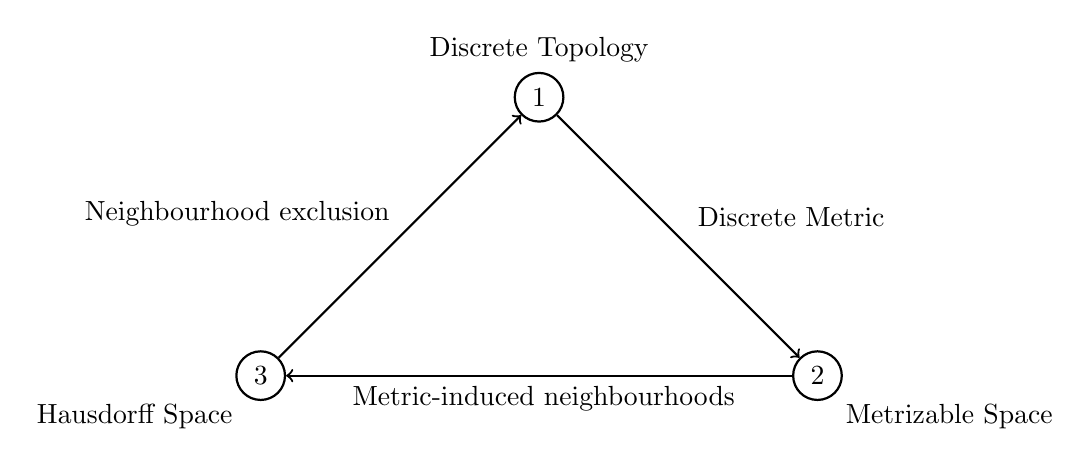
\begin{tikzpicture}[node distance={5cm}, thick, main/.style = {draw, circle}]
        \node[main, label=above:Discrete Topology] (1)                      {\(1\)};
        \node[main, label=below right:Metrizable Space] (2) [below right of=1]    {\(2\)};
        \node[main, label=below left:Hausdorff Space] (3) [below left of=1]      {\(3\)};

        % \pause

        \draw[->] (1) -- node[midway, above right] {\(\checkmark\) Discrete Metric} (2);
        \draw[->] (2) -- node[midway, below] {\(\checkmark\) Metric-induced neighbourhoods} (3);
        \draw[->] (3) -- node[midway, above left] {\(\checkmark\) Neighbourhood exclusion} (1);

    \end{tikzpicture}

\end{frame}